% Options for packages loaded elsewhere
\PassOptionsToPackage{unicode}{hyperref}
\PassOptionsToPackage{hyphens}{url}
%
\documentclass[
]{article}
\usepackage{amsmath,amssymb}
\usepackage{lmodern}
\usepackage{iftex}
\ifPDFTeX
  \usepackage[T1]{fontenc}
  \usepackage[utf8]{inputenc}
  \usepackage{textcomp} % provide euro and other symbols
\else % if luatex or xetex
  \usepackage{unicode-math}
  \defaultfontfeatures{Scale=MatchLowercase}
  \defaultfontfeatures[\rmfamily]{Ligatures=TeX,Scale=1}
\fi
% Use upquote if available, for straight quotes in verbatim environments
\IfFileExists{upquote.sty}{\usepackage{upquote}}{}
\IfFileExists{microtype.sty}{% use microtype if available
  \usepackage[]{microtype}
  \UseMicrotypeSet[protrusion]{basicmath} % disable protrusion for tt fonts
}{}
\makeatletter
\@ifundefined{KOMAClassName}{% if non-KOMA class
  \IfFileExists{parskip.sty}{%
    \usepackage{parskip}
  }{% else
    \setlength{\parindent}{0pt}
    \setlength{\parskip}{6pt plus 2pt minus 1pt}}
}{% if KOMA class
  \KOMAoptions{parskip=half}}
\makeatother
\usepackage{xcolor}
\usepackage[margin=1in]{geometry}
\usepackage{longtable,booktabs,array}
\usepackage{calc} % for calculating minipage widths
% Correct order of tables after \paragraph or \subparagraph
\usepackage{etoolbox}
\makeatletter
\patchcmd\longtable{\par}{\if@noskipsec\mbox{}\fi\par}{}{}
\makeatother
% Allow footnotes in longtable head/foot
\IfFileExists{footnotehyper.sty}{\usepackage{footnotehyper}}{\usepackage{footnote}}
\makesavenoteenv{longtable}
\usepackage{graphicx}
\makeatletter
\def\maxwidth{\ifdim\Gin@nat@width>\linewidth\linewidth\else\Gin@nat@width\fi}
\def\maxheight{\ifdim\Gin@nat@height>\textheight\textheight\else\Gin@nat@height\fi}
\makeatother
% Scale images if necessary, so that they will not overflow the page
% margins by default, and it is still possible to overwrite the defaults
% using explicit options in \includegraphics[width, height, ...]{}
\setkeys{Gin}{width=\maxwidth,height=\maxheight,keepaspectratio}
% Set default figure placement to htbp
\makeatletter
\def\fps@figure{htbp}
\makeatother
\setlength{\emergencystretch}{3em} % prevent overfull lines
\providecommand{\tightlist}{%
  \setlength{\itemsep}{0pt}\setlength{\parskip}{0pt}}
\setcounter{secnumdepth}{-\maxdimen} % remove section numbering
\ifLuaTeX
  \usepackage{selnolig}  % disable illegal ligatures
\fi
\IfFileExists{bookmark.sty}{\usepackage{bookmark}}{\usepackage{hyperref}}
\IfFileExists{xurl.sty}{\usepackage{xurl}}{} % add URL line breaks if available
\urlstyle{same} % disable monospaced font for URLs
\hypersetup{
  pdftitle={Gender bias in ADHD diagnosis},
  pdfauthor={Alexandra Rossy},
  hidelinks,
  pdfcreator={LaTeX via pandoc}}

\title{Gender bias in ADHD diagnosis}
\author{Alexandra Rossy}
\date{(11 décembre, 2022)}

\begin{document}
\maketitle

\begin{figure}
\centering

\includegraphics{/Users/alex-/Master/data sciences/datapractical/ADHD_woman.jpg}
\caption{@ADHD\_couple, instagram:
\url{https://www.instagram.com/p/CF7aB2NDL3j/?hl=fr}}
\end{figure}

\hypertarget{introduction}{%
\subsection{Introduction}\label{introduction}}

\begin{itemize}
\tightlist
\item
  fact
\item
  fact
\end{itemize}

\hypertarget{references}{%
\subsection{References}\label{references}}

\hypertarget{articles}{%
\subsubsection{Articles:}\label{articles}}

Hinshaw, S. P., Nguyen, P. T., O'Grady, S. M., \& Rosenthal, E. A.
(2022). Annual Research Review: Attention-deficit/hyperactivity disorder
in girls and women: underrepresentation, longitudinal processes, and key
directions. \emph{Journal of child psychology and psychiatry, and allied
disciplines}, 63(4), 484--496.

Slobodin, O. \& Davidovitch, M.(2019). Gender Differences in Objective
and Subjective Measures of ADHD Among Clinic-Referred Children.
\emph{Frontiers}.

\hypertarget{data}{%
\subsubsection{Data:}\label{data}}

\begin{itemize}
\tightlist
\item
  National Survey of Children's Health, Health Resources and Services
  Administration, Maternal and Child Health Bureau.
  \url{https://mchb.hrsa.gov/data/national-surveys}

  \begin{itemize}
  \tightlist
  \item
    \href{https://www.childhealthdata.org/browse/survey/allstates?q=9343\&g=1008\&a=18062\#}{Data
    table}
  \end{itemize}
\end{itemize}

\hypertarget{pictures}{%
\subsubsection{Pictures:}\label{pictures}}

\begin{itemize}
\tightlist
\item
  @ADHD\_couple on
  \href{https://www.instagram.com/p/CF7aB2NDL3j/?hl=f}{Instagram}
\end{itemize}

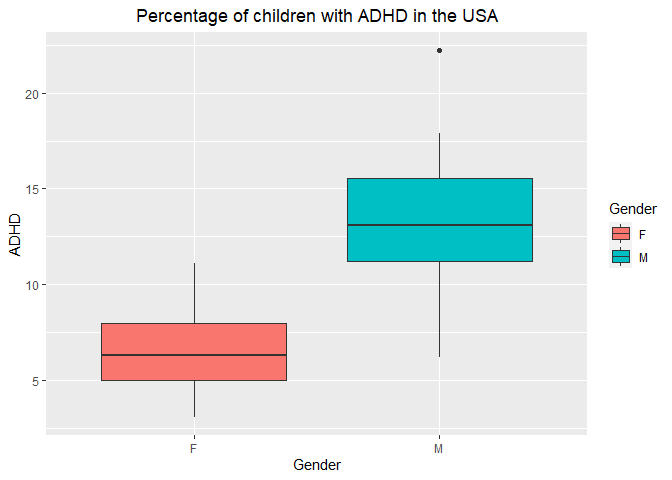
\includegraphics{datapractical_files/figure-latex/unnamed-chunk-2-1.pdf}

\begin{verbatim}
## 
##  Welch Two Sample t-test
## 
## data:  girls$ADHD and boys$ADHD
## t = -11.872, df = 83.933, p-value < 2.2e-16
## alternative hypothesis: true difference in means is not equal to 0
## 95 percent confidence interval:
##  -7.682649 -5.478135
## sample estimates:
## mean of x mean of y 
##  6.545098 13.125490
\end{verbatim}

\hypertarget{average-of-adults-with-adhd}{%
\subsubsection{Average of adults with
ADHD}\label{average-of-adults-with-adhd}}

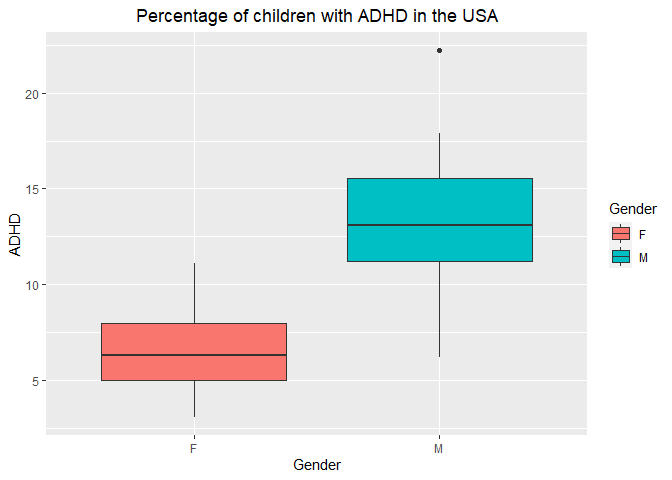
\includegraphics{datapractical_files/figure-latex/unnamed-chunk-3-1.pdf}

\begin{longtable}[]{@{}rr@{}}
\caption{Percentage of adult with ADHD in the USA}\tabularnewline
\toprule()
Women & Men \\
\midrule()
\endfirsthead
\toprule()
Women & Men \\
\midrule()
\endhead
3.2 & 5.4 \\
\bottomrule()
\end{longtable}

\begin{verbatim}
## 
##  One Sample t-test
## 
## data:  mean_adult
## t = 3.9091, df = 1, p-value = 0.1594
## alternative hypothesis: true mean is not equal to 0
## 95 percent confidence interval:
##  -9.676825 18.276825
## sample estimates:
## mean of x 
##       4.3
\end{verbatim}

\hypertarget{both-of-them}{%
\subsubsection{Both of them}\label{both-of-them}}

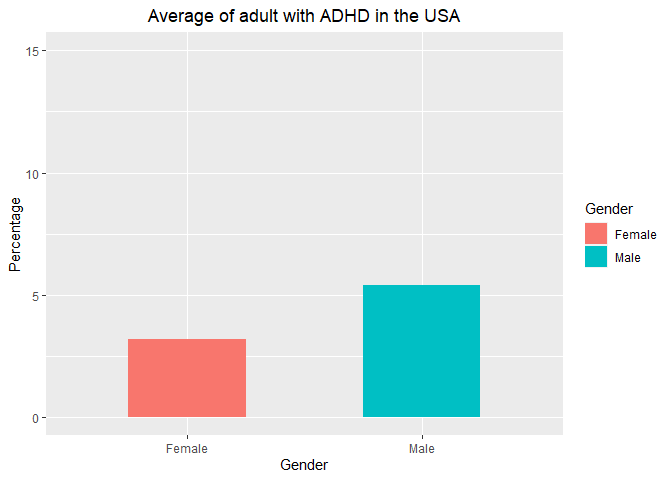
\includegraphics{datapractical_files/figure-latex/unnamed-chunk-4-1.pdf}

\begin{longtable}[]{@{}rr@{}}
\caption{Tab2: Average percentage of children with ADHD in the
USA}\tabularnewline
\toprule()
Girls & Boys \\
\midrule()
\endfirsthead
\toprule()
Girls & Boys \\
\midrule()
\endhead
6.545098 & 13.12549 \\
\bottomrule()
\end{longtable}

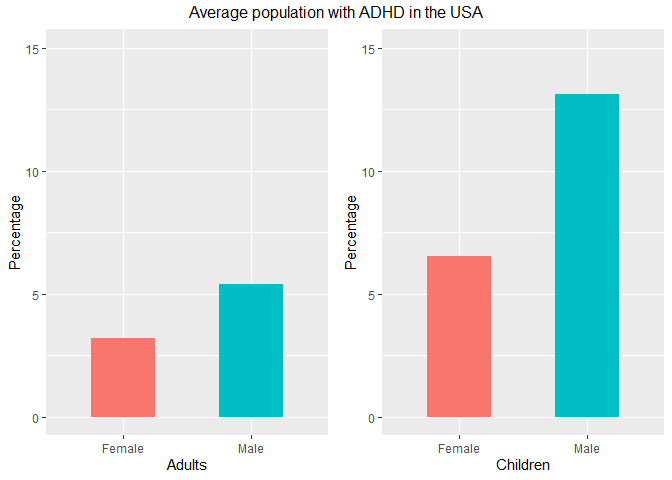
\includegraphics{datapractical_files/figure-latex/unnamed-chunk-4-2.pdf}
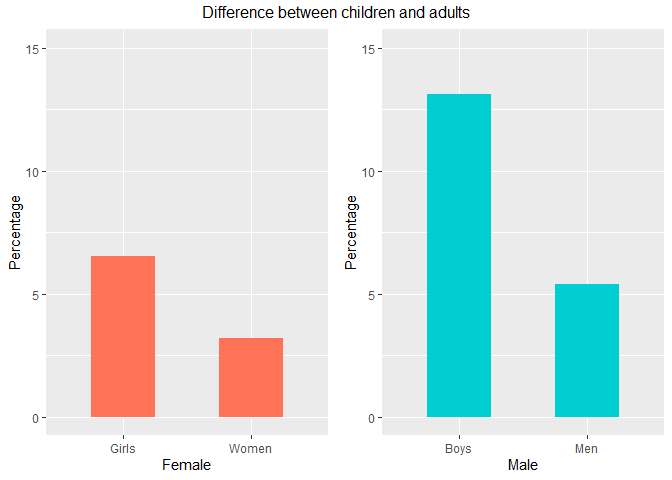
\includegraphics{datapractical_files/figure-latex/unnamed-chunk-4-3.pdf}

\begin{longtable}[]{@{}rrrr@{}}
\caption{Tab3: Average population with ADHD}\tabularnewline
\toprule()
Female & Male & Girls & Boys \\
\midrule()
\endfirsthead
\toprule()
Female & Male & Girls & Boys \\
\midrule()
\endhead
3.2 & 5.4 & 6.55 & 13.13 \\
\bottomrule()
\end{longtable}

\begin{longtable}[]{@{}ll@{}}
\caption{Percentage of adults who still have ADHD}\tabularnewline
\toprule()
Women & Men \\
\midrule()
\endfirsthead
\toprule()
Women & Men \\
\midrule()
\endhead
\textasciitilde{} 49\% & \textasciitilde{} 43\% \\
\bottomrule()
\end{longtable}

\hypertarget{trying-two-tab-side-by-side}{%
\subsubsection{Trying two tab side by
side}\label{trying-two-tab-side-by-side}}

\begin{longtable}[]{@{}rrrr@{}}
\caption{Tab3: Average population with ADHD}\tabularnewline
\toprule()
Female & Male & Girls & Boys \\
\midrule()
\endfirsthead
\toprule()
Female & Male & Girls & Boys \\
\midrule()
\endhead
3.2 & 5.4 & 6.55 & 13.13 \\
\bottomrule()
\end{longtable}

\begin{longtable}[]{@{}ll@{}}
\caption{Percentage of adults who still have ADHD}\tabularnewline
\toprule()
Women & Men \\
\midrule()
\endfirsthead
\toprule()
Women & Men \\
\midrule()
\endhead
\textasciitilde{} 49\% & \textasciitilde{} 43\% \\
\bottomrule()
\end{longtable}

\begin{table}
\caption{\label{tab:figure-side}Two tables placed side by side.}

\centering
\begin{tabular}[t]{rrrr}
\toprule
Female & Male & Girls & Boys\\
\midrule
3.2 & 5.4 & 6.55 & 13.13\\
\bottomrule
\end{tabular}
\centering
\begin{tabular}[t]{ll}
\toprule
Women & Men\\
\midrule
\textasciitilde{} 49\% & \textasciitilde{} 43\%\\
\bottomrule
\end{tabular}
\end{table}

\hypertarget{facts}{%
\subsubsection{Facts}\label{facts}}

``A meta-analysis of follow-up studies of children with ADHD found that
15\% continue to meet full diagnostic criteria at the age of 25 years,
with a further 50\% experiencing some degree of continued impairments
and subthreshold symptom''. So aound 65\%-70\% of the children diagnosed
will still have ADHD. For boys we expect around 4.6 percent and for
girls we expect around \ldots{} around 60\% for boys still with ADHD, in
women -\textgreater{} almost 70\% still! so means that maybe some women
diagnosed later.

If we take it for the data of 2006, for men with ADHD we can see that we
still have

\hypertarget{trying-time-series}{%
\subsubsection{Trying time series}\label{trying-time-series}}

\begin{verbatim}
## 
##  Welch Two Sample t-test
## 
## data:  male_tab$Percentage and female_tab$Percentage
## t = 1.0422, df = 1.3628, p-value = 0.4473
## alternative hypothesis: true difference in means is not equal to 0
## 95 percent confidence interval:
##  -24.85411  33.63411
## sample estimates:
## mean of x mean of y 
##     9.265     4.875
\end{verbatim}

\end{document}
